\documentclass[12pt,a4paper,oneside,final]{article}

\usepackage[utf8]{inputenc}
\usepackage{amsmath,amssymb,amsfonts}
\usepackage{bm}
\usepackage[hidelinks]{hyperref}

\usepackage[margin=1in]{geometry}
\usepackage{listings}
\usepackage{fancyhdr}
\usepackage{lastpage}
\usepackage{titlesec}

\usepackage{float}
\usepackage{graphicx}
\usepackage{caption}
\usepackage{subcaption}
\usepackage[section]{placeins}
\usepackage{color}

\pagestyle{fancy}
\addtolength{\headheight}{\baselineskip}
\setcounter{secnumdepth}{4}
\setcounter{tocdepth}{1}

\rhead{Vision and image processing \\ Assignment 3, 08/01-18}
\lhead{Therese Darum, zbl558; Cecilie Novak, bk662; \\ Christoffer Belhage, DZP300}
\cfoot{Page \thepage\ of \pageref{LastPage}}

\begin{document}

\section{Programming language and libraries used}
For this assignment \texttt{Matlab} and its \texttt{Image processing toolbox} have been used.

\section{Assumptions, method used and implementation}

\subsection{Assumptions made}
We have made some assumptions about the input images in order to make the code handed in for this assignment. These are as follows:
\begin{itemize}
\item[-] The input images are assumed to be rectified beforehand.
\item[-] We assume that image objects moves to the right in the second image.  That is, we do not accept negative disparities (corresponding to image objects moving to the left in the images), as the scene should only be moving in one direction.
\item[-] We assume that disparities should be calculated using intensity images - in contrast to the input images that are given as colour images. The images will therefore automatically be converted from colour images to intensity images using the built-in Matlab method \texttt{rgb2gray}.
\end{itemize}

\subsection{Method used}
The method applied for calculating the disparity from the rectified images is based on gaussian pyramids. A coarse disparity was first calculated using the top scale of the gaussian pyramid (the smallest image). The disparities were then iteratively corrected to increase precision when moving down through the scales in the gaussian pyramid, by doubling the disparities before adding them to the disparities calculated from the next scale. \\\\
This way, we do not need to search the whole horizontal line, on which matching pixels can lie on, as we narrow down the place where we expect the pixels to be found, given the disparities in the previous scale (as in the scale above the current scale).\\\\
The actual disparity in any given scale, was calculated based on the normalized cross-correlation. The first pixel with the highest normalized cross-correlation to the right of any given pixel was used as match for any pixel, that is, we have used one-way matching, not two-way matching. We have not made use of any corrections for the discontinuities in the disparities, as suggested in the assignment text (due to lack of time). \\\\
We have not computed a full gaussian pyramid for the disparity calculations, but only uses up to 4 scales (as adviced in the assignment text), which might affect the calculations of the disparity, as we do not start at the smallest scale possible.

\section{The implementation}
We have used some built-in methods for essential parts of the program. First up, we used Matlab's \texttt{impyramid} method in order to create the different scales of the gaussian pyramid. This function applies a slight blur to the image (something similar to a gaussian blur), then downsizes the image to half height and width.\\\\
Secondly, we used Matlab's \texttt{normxcorr2} method for calculating the normalized cross-correlation between a template and a horizontal fragment of the target image - the search area. Unfortunately, this was an unwise decision, as it also calculates all horizontal correlations (i.e. having the template partially above or below the center line of the search area). This uses up a large, and completely unnecessary, amount of computing power.\\\\
Ignoring that, our program works by taking any pre-calculated disparities (from higher scale levels in the gaussian pyramid), and using corresponding disparities for a given pixel to determine where to center the search area. Once a search area is chosen, we use the normalized cross-correlation function to determine which pixel on the same horizontal line is the best match, using a patch around the original pixel location as template. The difference between the original location and the best matching pixel is then recorded as the disparity for that pixel.\\\\
The cross-correlation function also compares the patch with the search area such that the patch only partially overlaps with the search area (at the edges). We have chosen to ignore such comparisons, as they may have a very high correlation, but are obviously wrong (according to tests that we made). Therefore the disparities near the left edge of the image are all zero; Which also makes some sense, as we in truth do not know what would lie outside of the image.

\section{Testing and results}

\subsection{Methods}
We spent a lot of time debugging our code; The most effective ways that we tested our implementation was by using small fragments of pictures shifted a couple of pixels. That way we knew what the expected result should be, and was able to verify if the code worked as intended.\\\\
Once we had working code up and running, we used the sample images to optimize our methods to get better results. Some of these optmizations included tweaking the search area for the cross-correlation and discarding the parts of the search area on the left side of the template (see description in previous section for details).\\\\
When we had implemented our optimizations we performed a parameter test; That is, we varied the template size, and the number of scales used. Results are shown in the next section.

\subsection{Results}
\begin{figure}[H]
\centering
\begin{subfigure}[b]{0.24\textwidth}
	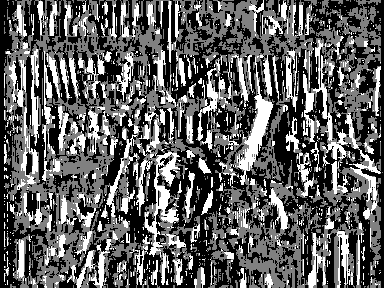
\includegraphics[width=\textwidth]{disparity_s1_k5.png}
	\caption{Template size = 5, 1 scale.}
\end{subfigure}
\begin{subfigure}[b]{0.24\textwidth}
	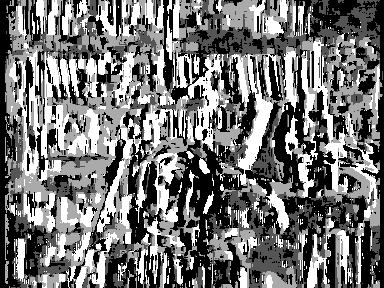
\includegraphics[width=\textwidth]{disparity_s1_k7.png}
	\caption{Template size = 7, 1 scale.}
\end{subfigure}
\begin{subfigure}[b]{0.24\textwidth}
	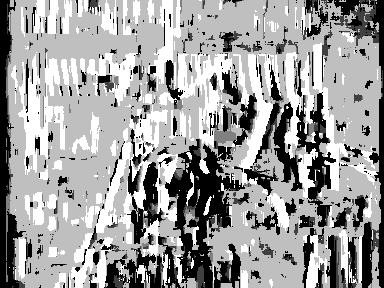
\includegraphics[width=\textwidth]{disparity_s1_k9.png}
	\caption{Template size = 9, 1 scale.}
\end{subfigure}
\begin{subfigure}[b]{0.24\textwidth}
	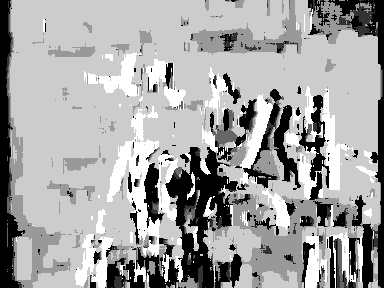
\includegraphics[width=\textwidth]{disparity_s1_k11.png}
	\caption{Template size = 11, 1 scale.}
\end{subfigure}
\end{figure}
\begin{figure}[H]
\ContinuedFloat
\begin{subfigure}[b]{0.24\textwidth}
	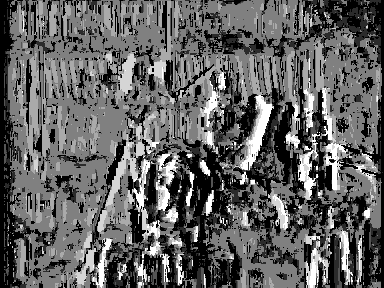
\includegraphics[width=\textwidth]{disparity_s2_k5.png}
	\caption{Template size = 5, 2 scales.}
\end{subfigure}
\begin{subfigure}[b]{0.24\textwidth}
	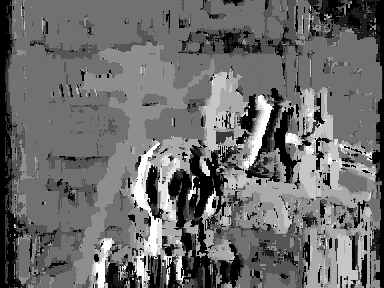
\includegraphics[width=\textwidth]{disparity_s2_k7.png}
	\caption{Template size = 7, 2 scales.}
\end{subfigure}
\begin{subfigure}[b]{0.24\textwidth}
	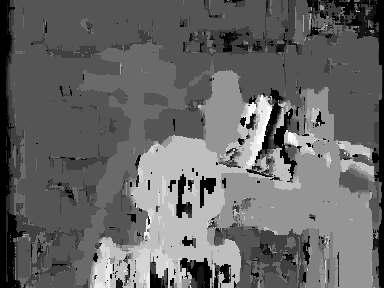
\includegraphics[width=\textwidth]{disparity_s2_k9.png}
	\caption{Template size = 9, 2 scales.}
\end{subfigure}
\begin{subfigure}[b]{0.24\textwidth}
	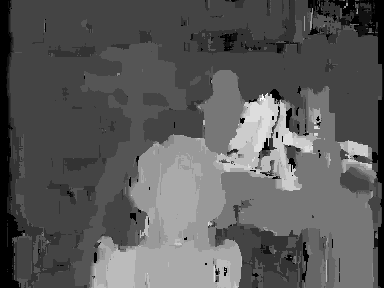
\includegraphics[width=\textwidth]{disparity_s2_k11.png}
	\caption{Template size = 11, 2 scales.}
\end{subfigure}
\end{figure}
\begin{figure}[H]
\ContinuedFloat
\begin{subfigure}[b]{0.24\textwidth}
	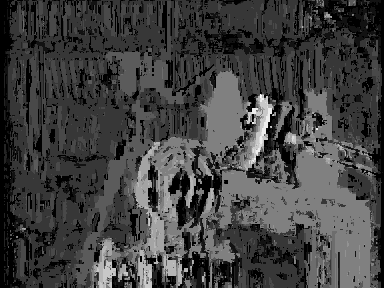
\includegraphics[width=\textwidth]{disparity_s3_k5.png}
	\caption{Template size = 5, 3 scales.}
\end{subfigure}
\begin{subfigure}[b]{0.24\textwidth}
	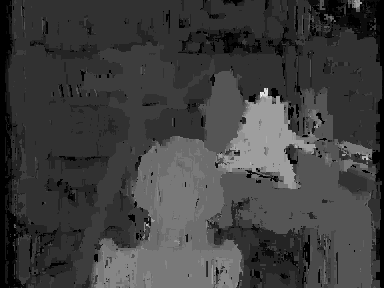
\includegraphics[width=\textwidth]{disparity_s3_k7.png}
	\caption{Template size = 7, 3 scales.}
\end{subfigure}
\begin{subfigure}[b]{0.24\textwidth}
	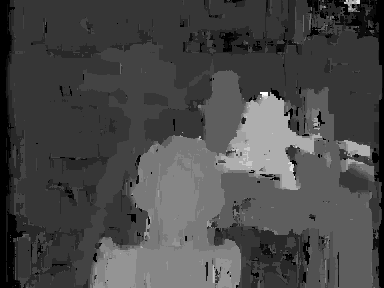
\includegraphics[width=\textwidth]{disparity_s3_k9.png}
	\caption{Template size = 9, 3 scales.}
\end{subfigure}
\begin{subfigure}[b]{0.24\textwidth}
	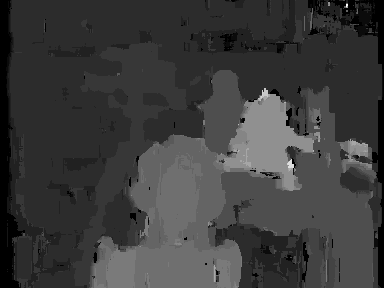
\includegraphics[width=\textwidth]{disparity_s3_k11.png}
	\caption{Template size = 11, 3 scales.}
\end{subfigure}
\end{figure}
\begin{figure}[H]
\ContinuedFloat
\begin{subfigure}[b]{0.24\textwidth}
	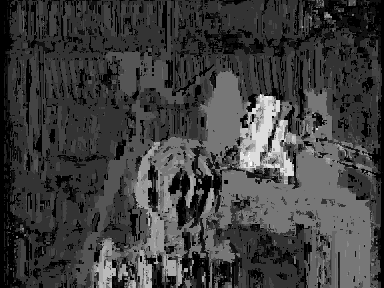
\includegraphics[width=\textwidth]{disparity_s4_k5.png}
	\caption{Template size = 5, 4 scales.}
\end{subfigure}
\begin{subfigure}[b]{0.24\textwidth}
	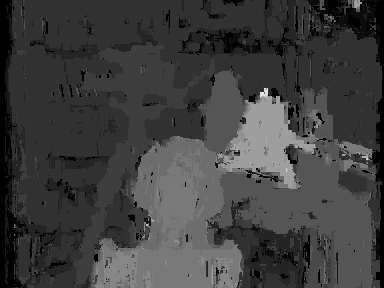
\includegraphics[width=\textwidth]{disparity_s4_k7.png}
	\caption{Template size = 7, 4 scales.}
\end{subfigure}
\begin{subfigure}[b]{0.24\textwidth}
	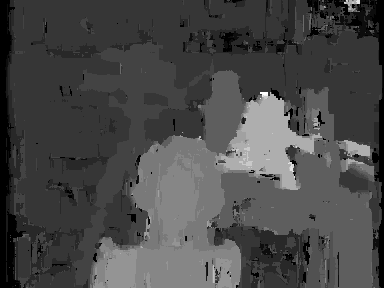
\includegraphics[width=\textwidth]{disparity_s4_k9.png}
	\caption{Template size = 9, 4 scales.}
\end{subfigure}
\begin{subfigure}[b]{0.24\textwidth}
	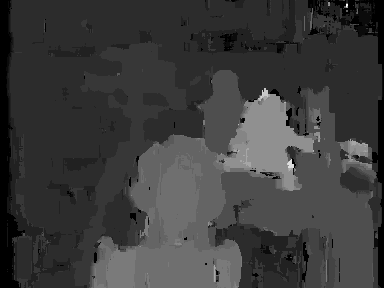
\includegraphics[width=\textwidth]{disparity_s4_k11.png}
	\caption{Template size = 11, 4 scales.}
\end{subfigure}
\caption{Disparities calculated by varying the number of used scales from the gaussian pyramid and template size.}
\label{fig:disparities}
\end{figure}

In figure \ref{fig:disparities} we see the resulting disparity images for different numbers of scale levels and kernel sizes. There are a few things to take away from this: Template size means a lot for the quality of the result. With the lower size templates, there are a lot of "holes". This could be due to the search area being scaled according to the template size; A deliberate choice, but in retrospect it may have been better to choose a fixed size for the search area across all templates, the reason being that smaller templates may result in such a narrow search area that the true match is outside of the search area and thus not able to be matched correctly.\\\\
Then one would expect that any additional scale levels would "fix" the issue - However this does not seem to be the case when looking at the difference between scales levels 3 and 4 with template size 5. There is only a slight difference and that is on the lamp. It makes sense that there would be a difference there, as it is the part of the image that changes the most.\\\\
\iffalse
{\color{red} It is pretty obvoius when looking at the lower level disparities in figure \ref{fig:lowlevel}:
\begin{figure}[H]
\centering
\begin{subfigure}[b]{0.24\textwidth}
	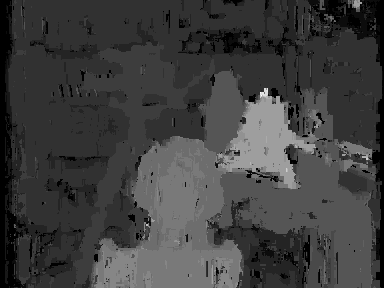
\includegraphics[width=\textwidth]{disparity1.png}
	\caption{Scale level 1.}
\end{subfigure}
\begin{subfigure}[b]{0.24\textwidth}
	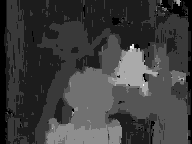
\includegraphics[width=\textwidth]{disparity2.png}
	\caption{Scale level 2.}
\end{subfigure}
\begin{subfigure}[b]{0.24\textwidth}
	
\includegraphics[width=\textwidth]{disparity3.png}
	\caption{Scale level 3.}
\end{subfigure}
\begin{subfigure}[b]{0.24\textwidth}
	
\includegraphics[width=\textwidth]{disparity4.png}
	\caption{Scale level 4.}
\end{subfigure}
\caption{The disparity of different scales (using kernel size 7). Higher resolution scales are based on lower resolution scales.}
\label{fig:lowlevel}
\end{figure}
While the disparity images in figure \ref{fig:lowlevel} are for template size 7, and not 5, it still shows why adding the last scale added quality to the lamp area, but why the rest of the image (for kernel size 5) is still not filled out is puzzling.}
\fi
Another fact we see from the tests is that larger templates improve quality (probably with diminishing returns); However, increased template size also means more computation - Especially in our implementation where search area scales with the template size and because of our use of \texttt{normxcorr2}. It also means higher risk of false positive matchings and more errors at the boundary of objects due to stronger occlusion effects.\\\\
\iffalse
{\color{red}
Lastly, adding a level of scale only add benefits to a certain level; In most cases we see little to no improvement in quality when adding the fourth scale. Maybe with an even smaller search area, extra scale levels would make sense, but they are already fairly small. }
\fi

\begin{table}[H]
	\centering
	\begin{subtable}{1\textwidth}
		\centering
		\begin{tabular}{c||c|c|c|c}
			Template size &5&7&9&11\\\hline
			Mean error &91.676&97.717&115.279&111.623\\\hline
			Standard deviation &65.013&68.073&60.596&56.912\\\hline
			\# large errors &94909&100633&102920&103469\\\hline
			Fraction of large errors &0.858&0.910&0.931&0.936\\\hline
		\end{tabular}
		\caption{Calculated with 1 scale level.}
	\end{subtable}
	\begin{subtable}{1\textwidth}
		\centering
		\begin{tabular}{c||c|c|c|c}
			Template size &5&7&9&11\\\hline
			Mean error &74.837&56.363&44.580&39.742\\\hline
			Standard deviation &52.439&48.593&45.825&48.161\\\hline
			\# large errors &99558&104528&105233&105104\\\hline
			Fraction of large errors &0.900&0.945&0.952&0.950\\\hline
		\end{tabular}
		\caption{Calculated with 2 scale levels.}
	\end{subtable}
	\begin{subtable}{1\textwidth}
		\centering
		\begin{tabular}{c||c|c|c|c}
			Template size &5&7&9&11\\\hline
			Mean error &48.247&36.777&36.308&35.465\\\hline
			Standard deviation &47.984&46.246&47.266&47.107\\\hline
			\# large errors &102891&72908&70614&68582\\\hline
			Fraction of large errors &0.930&0.659&0.639&0.620\\\hline
		\end{tabular}
		\caption{Calculated with 3 scale levels.}
	\end{subtable}
	\begin{subtable}{1\textwidth}
		\centering
		\begin{tabular}{c||c|c|c|c}
			Template size &5&7&9&11\\\hline
			Mean error &44.388&36.760&36.315&35.468\\\hline
			Standard deviation &43.555&46.222&47.271&47.106\\\hline
			\# large errors &92788&72893&70616&68591\\\hline
			Fraction of large errors &0.839&0.659&0.639&0.620\\\hline
		\end{tabular}
		\caption{Calculated with 4 scale levels.}
	\end{subtable}
	\caption{Numerical evaluation of results}
	\label{tab:numeval}
\end{table}
In table \ref{tab:numeval} we see a numerical evaluation of our results, for varying number of scale levels and template sizes. From the tables we can see that for all number of scale levels the mean error goes down when the template size goes up. This is sound, since small patches are more likely to match many places in the image, because of the simple structure. Larger patches have a more complex structure, and thus are more difficult to match (and thus more difficult to match wrongly). Number of scale levels also seem to have a great impact on the mean error.\\\\
The standard deviation of the error does not seem to depend greatly on the template size, but still there is a slight tendency for the standard deviation to become smaller when the number of scales goes up.\\\\
For few scale levels we seem to get fewer large errors when the template size is small, but as soon as we have more than 2 levels, we also need larger templates. We get the overall best results when we use 4 scales levels. \\\\
Figure \ref{fig:error} visualize the difference in the ground truth and the calculated disparities, for different template sizes and 4 scale levels. As suspected we get the most errors for kernel size 5, after which the errors gradually disappears. Looking at figure \ref{fig:error}d, which we read from the tables to be the combination with least large errors, we see that most of the errors that we get are around the objects, namely pixels becoming obscured or cease being obscured. We also see large errors on the borders, which in the ground truth image have been manually set to 0. We have not done so, hence the errors on the borders.

\begin{figure}[H]
	\centering
	\begin{subfigure}[b]{0.5\textwidth}
		\centering
		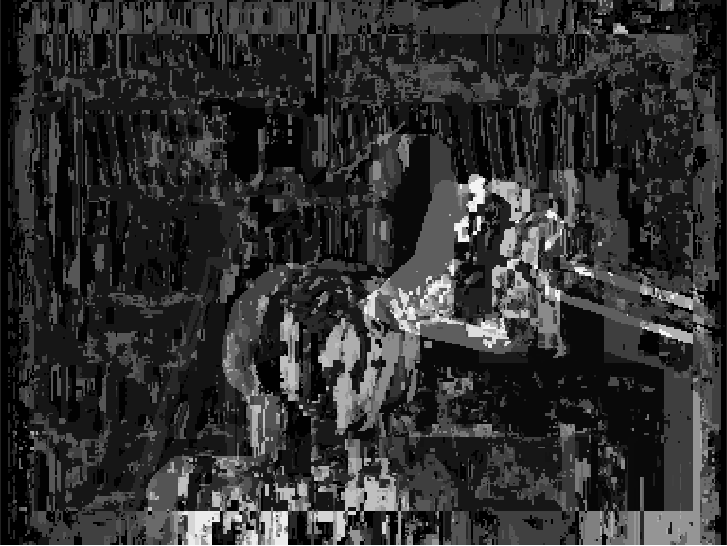
\includegraphics[width=7cm]{errk5.png}
		\caption{Template size 5.}
	\end{subfigure}%
	\begin{subfigure}[b]{0.5\textwidth}
		\centering
		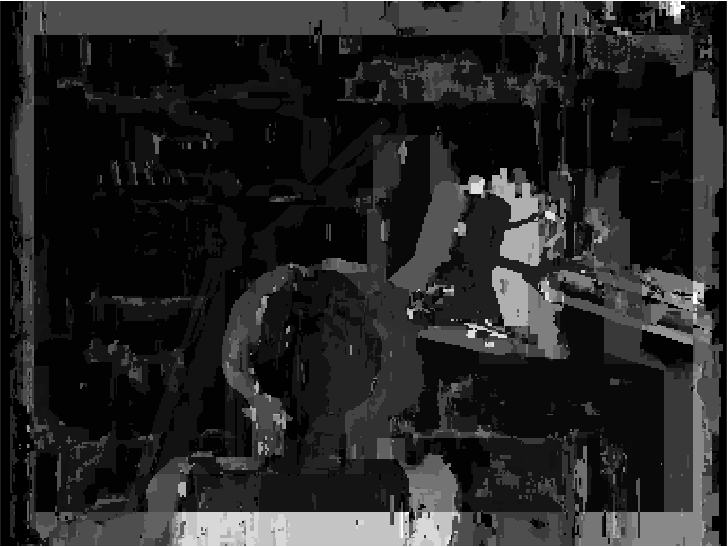
\includegraphics[width=7cm]{errk7.png}
		\caption{Template size 7.}
	\end{subfigure}
	\begin{subfigure}[b]{0.5\textwidth}
		\centering
		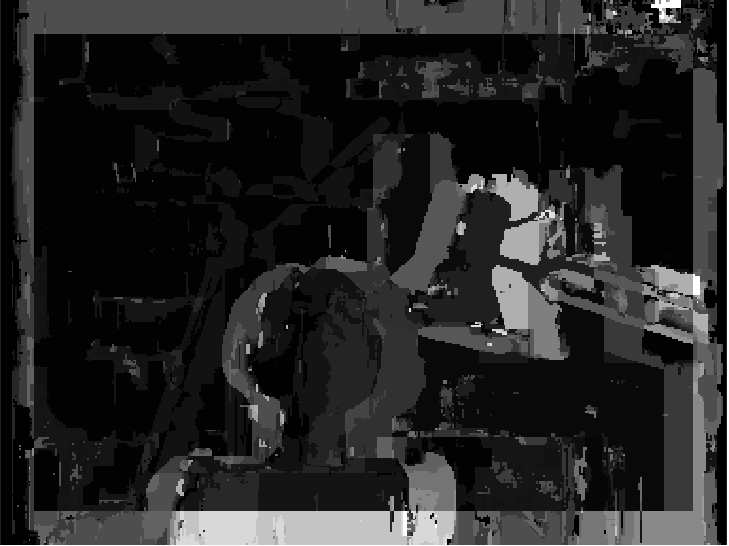
\includegraphics[width=7cm]{errk9.png}
		\caption{Template size 9.}
	\end{subfigure}%
	\begin{subfigure}[b]{0.5\textwidth}
		\centering
		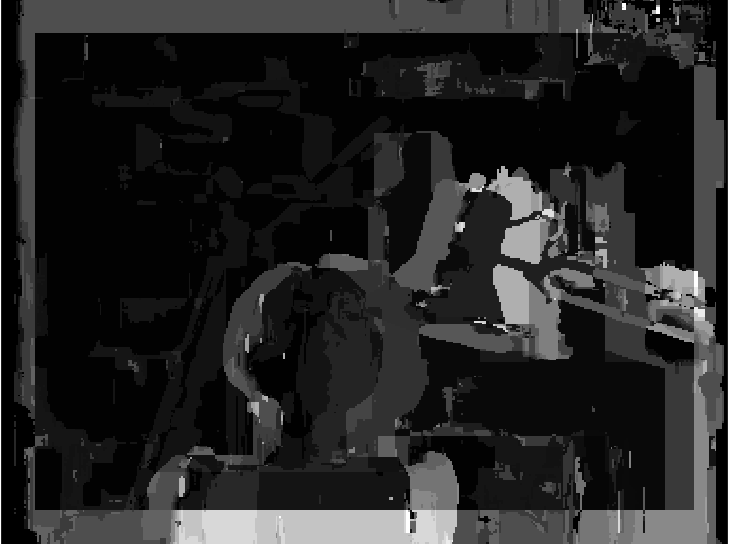
\includegraphics[width=7cm]{errk11.png}
		\caption{Template size 11.}
	\end{subfigure}
	\caption{The error for different Template sizes and 4 scale levels.}
	\label{fig:error}
\end{figure}

Looking at figure \ref{fig:disparities}p, again the disparity calculation which we read from the tables to be our most successful result, we see that we got most of it right. Form our calculations the lamp is closest to us, following part of the bust's face, the rest of the bust, the table and everything on it, then the camera and lastly the bookcase in the background. This is exactly the order we see in the ground truth image, though our edges are not quite as smooth, and as we already mentioned we have a problem with the discontinuities("holes"). However we are still able to recognize the shapes of the objects in the image. 

\subsection{Remark on results}
Part of the reason why we get so many errors might be because the values of the ground truth and our calculations might be scaled differently. Despite the errors, we believe overall that we have successfully provided depth information that mostly consists with what we see in the ground truth image.

\end{document}